\section{Grundlagen}

In diesem Kapitel werden die Grundlagen dieser Arbeit beschrieben. Dazu gehören unter anderem einige technischen Details über KDE, Wissenswertes über die Versionshistorie, sowie der aktuelle Stand des Projekts.

\subsection{Übersicht}
In der heutigen Computerwelt ist die Interaktion zwischen Mensch und Computer ohne eine graphische Benutzeroberfläche nahezu undenkbar. Daher gibt es eine große Auswahl an unterschiedlichen Betriebssystemen, die auch unterschiedliche Benutzeroberflächen haben. Eines dieser graphischen Benutzeroberflächen ist KDE.

\begin{figure}[h]
	\centering
	
\includegraphics[width=0.7\linewidth]{images/KDE_logo.png}
	\caption{Aktuelles offizielles KDE Logo. \cite{kdelogo}}
	\label{fig:kdelogo}
\end{figure}

KDE stand ursprünglich für \textit{Kool Desktop Environment} und steht heute für \textit{K Desktop Environment}, zu deutsch \textit{K Arbeitsumgebung}, wobei das \textit{K} keine bestimmte Bedeutung mehr hat, sondern als eine Art Markenzeichen von KDE ist. Es handelt sich dabei um eine graphische Arbeitsumgebung für UNIX-Betriebssysteme. Es besteht aus einer Reihe von kleinen Programmen, einem Fenstermanager, einem Dateimanager und einigen Hilfsprogrammen. Das Ziel von KDE ist es, die Verwendung von UNIX-basierten Betriebssystemen zu vereinfachen. \cite{TUChemnitzKDE}. Bild \ref{fig:kdelogo} zeigt das aktuelle offizielle KDE Logo.

\subsection{Versionshistorie}
Das KDE Projekt wurde am 14. Oktober 1996 von Matthias Ettrich begonnen. Sowohl der Name also auch der Funktionsumfang des Projekts orientierte sich an der proprietäre Desktop-Umgebung CDE (\textit{Common Desktop Environment}). KDE setzte von Beginn an auf die Programmiersprache C++ und auf die umfangreiche Oberflächenbibliothek \textit{Qt}.

\subsubsection{KDE 1.x}
Die KDE-Komponenten wurden ziemlich unkoordiniert entwickelt, weshalb es keine einheitlichen Alpha-Version gab. Etwa ein Jahr nach der Gründung von KDE erschien am 20. Oktober 1997 die erste Beta-Version. Nach drei weiteren Beta-Versionen wurde am 12. Juli 1998 die Version 1.0 von KDE präsentiert und veröffentlicht. Abbildung \ref{fig:kdeversion1} zeigt einen Standbild der Benutzeroberfläche von K Desktop Environments Version 1.0. Trotz einiger Kritik wegen der unfreien Bibliothek Qt konnte sie sich durchsetzen und fand seinen weg in einige Linux-Distributionen. \cite{kdeversion1}

\begin{figure}[h]
	\centering
	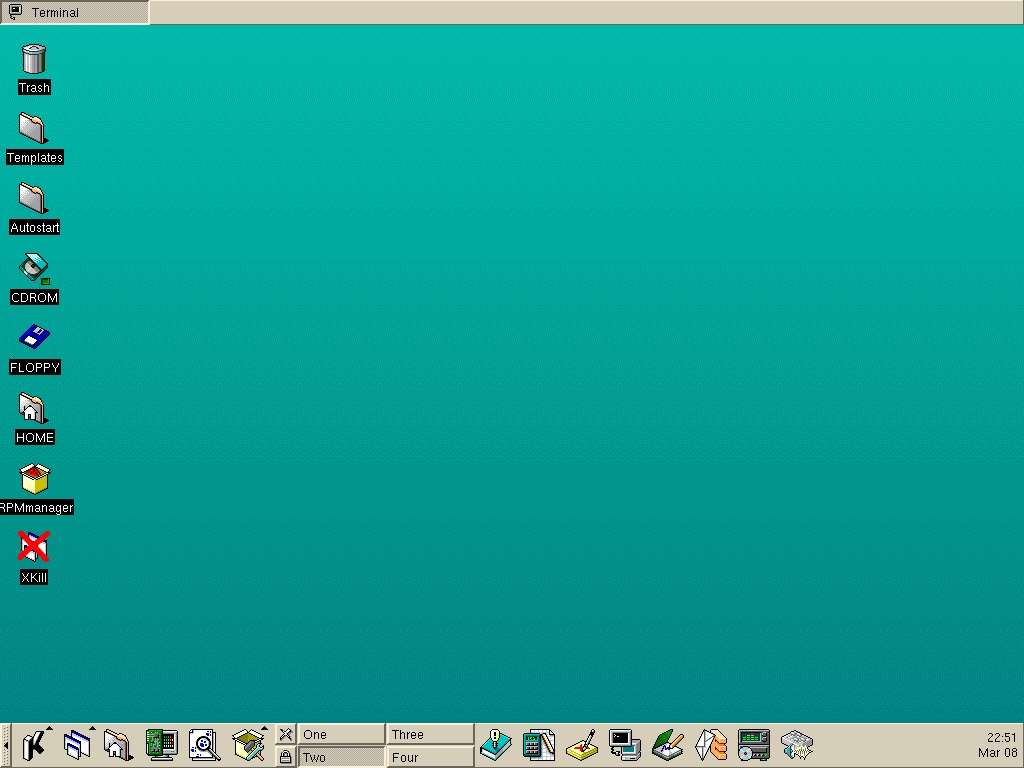
\includegraphics[width=\linewidth]{images/KDE_1.png}
	\caption{KDE Version 1.0 \cite{kdeversionenwiki}}
	\label{fig:kdeversion1}
\end{figure}

In den folgenden beiden Jahren wurde KDE durch zahlreiche Verbesserungen in einigen Punkten den Wünschen von Nutzern angepasst und auf die Version 1.1 gebracht. Durch eine neue Version der Oberflächenbibliothek Qt stand KDE vor vielen Verbesserungen, weshalb man sich entschied, die Verbesserungen nicht in die erste Generation von KDE aufzunehmen. Dieser Versionssprung wurde dazu genutzt die unkoordinierte Entwicklung und die Infrastruktur des Projekts zu überarbeiten. Bis zu Veröffentlichung wurde auch Qt unter die Lizenz GPL 2.0 gestellt, wodurch der Lizenzkonflikt zwischen den Lizenzen von KDE und Qt behoben wurde.

\subsubsection{KDE 2.x}
Die stabile Version von K Desktop Environments 2.0 wurde schließlich am 23. Oktober 2000 veröffentlicht. Abgesehen von den der besseren Infrastruktur wurde diese Version nun mit der freien Bibliothek Qt 2.2 veröffentlicht. Des Weitere erntete auch \textit{Konqueror}, der neue KDE-Dateimanager und -Webbrowser, viel positive Kritik. Andere Websbrowser waren zu dieser Zeit sehr unstabil oder nicht fertiggestellt. Abbildung \ref{fig:kdeversion2} zeigt die Benutzeroberfläche von K Desktop Environments 2 und den Webbrowser Konqueror. Durch KDE 2.0 konnte sich das Unternehmen als feste Institution unter den X11-Oberflächen durchsetzen. \cite{kdeversionenwiki, geschichtekde}

\begin{figure}[h]
	\centering
	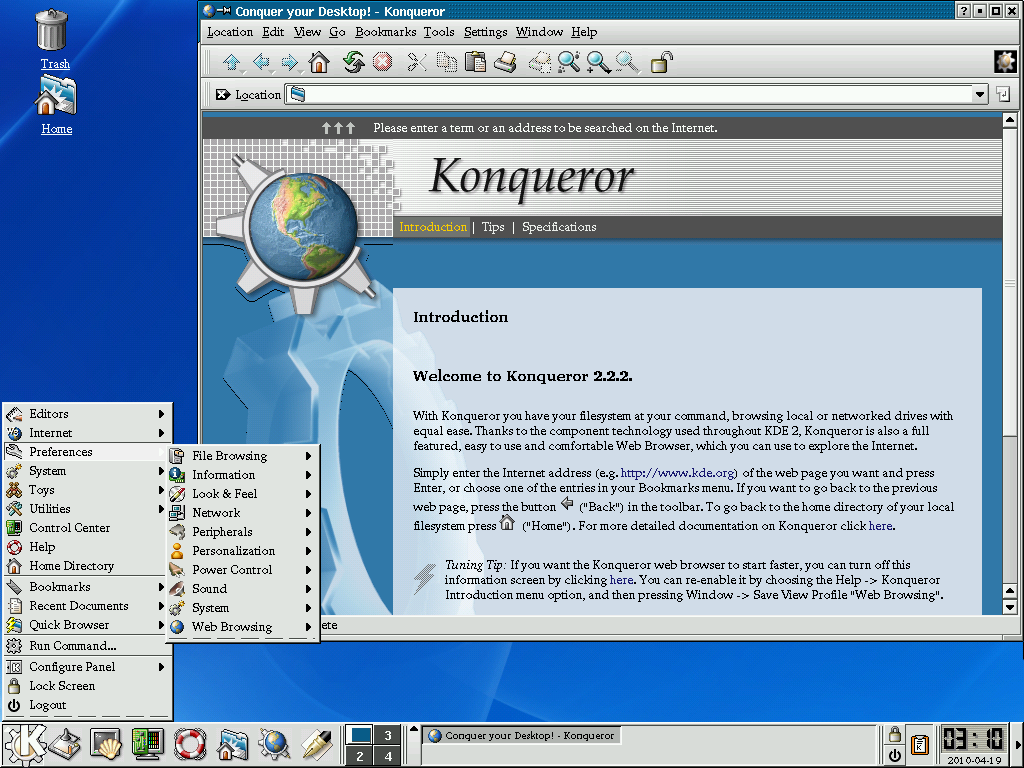
\includegraphics[width=\linewidth]{images/KDE_222.png}
	\caption{KDE Version 2.2.2 \cite{kdeversionenwiki}}
	\label{fig:kdeversion2}
\end{figure}

\subsubsection{KDE 3.x}
Nach zahlreichen Verbesserungen und zwei weiteren Veröffentlichungen von KDE in der zweiten Generation erschien am 3. April 2002 die Version 3.0. Diese und die darauffolgenden Versionen der 3. Generation brachten viele Neuerungen. Dazu zählten beispielsweise das \textit{Desktop Sharing Framework}, wodurch KDE-Desktops von entfernten Rechner verwendet werden konnten, \textit{Tabbed Browsing} in Konqueror und einen integrierten \textit{Personal Information Manager} namens \textit{Kontact}, das in einer Anwendung nützliche Funktionen wie E-Mail, Adressbuch, Kalender, Terminplaner, Newsreader, Wetteranzeige, Geburtstagserinnerung, Notizblock und Aufgabenliste kombinierte. Außerdem wurde der Benutzeroberfläche durch überarbeitete Icons und (in einigen Bereichen) durch neuem Design ein modernes Aussehen verliehen. \cite{kdeversionenwiki, geschichtekde} In Abbildung \ref{fig:kdeversion3} ist K Desktop Environments in der Version 3.5 zu sehen.

\begin{figure}[h]
	\centering
	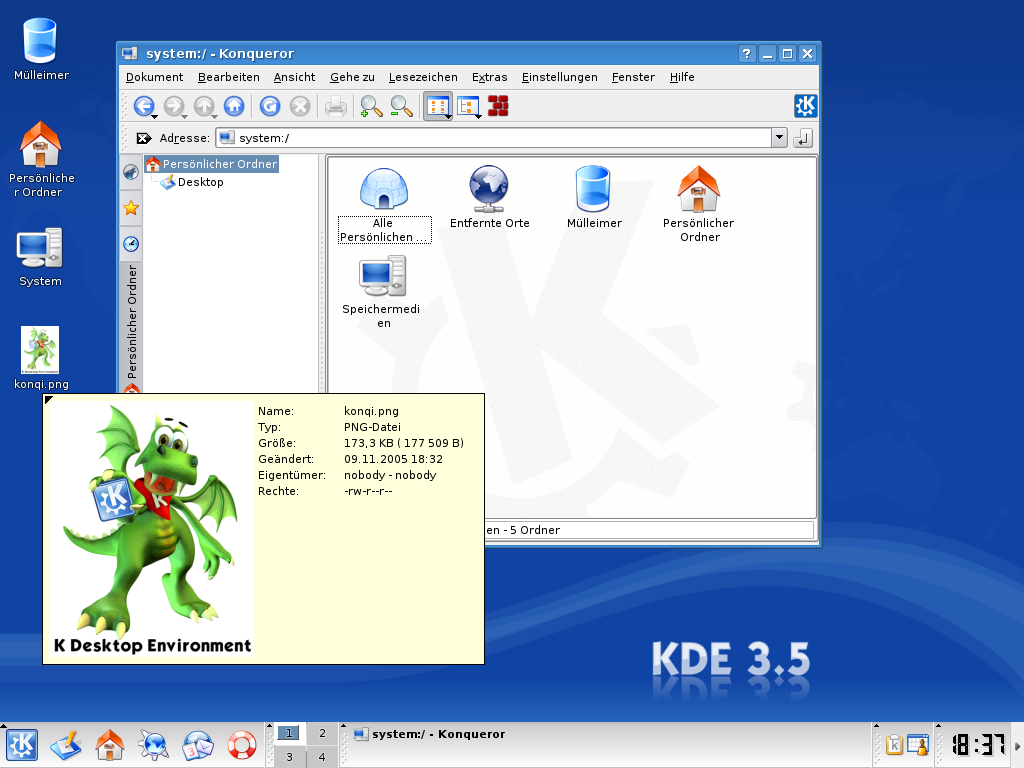
\includegraphics[width=\linewidth]{images/KDE_35.png}
	\caption{KDE Version 3.5 \cite{kdeversionenwiki}}
	\label{fig:kdeversion3}
\end{figure}

\subsubsection{KDE Plasma Workspaces 4}
In der darauffolgenden Version wurde die Ausformulierung K Desktop Environments nicht mehr verwendet und es erschien am  11. Januar 2008 KDE 4. Es wurde auf Basis von Qt 4 entwickelt. Viele Teile von KDE wurden von Grund auf neu programmiert, wie etwa der Desktop Plasma, also die Desktopumgebung und KDE. Zusammen mit KDE 4.2 wurden alle Funktionen aus KDE 3.x portiert und die Software war so stabil, dass die Nutzung von ihr erstmals auch für Endanwender empfohlen wurde. \cite{geschichtekde} Abbildung \ref{fig:kdeversion4} zeigt die Benutzeroberfläche von KDE in der Version 4.2.

\begin{figure}[h]
	\centering
	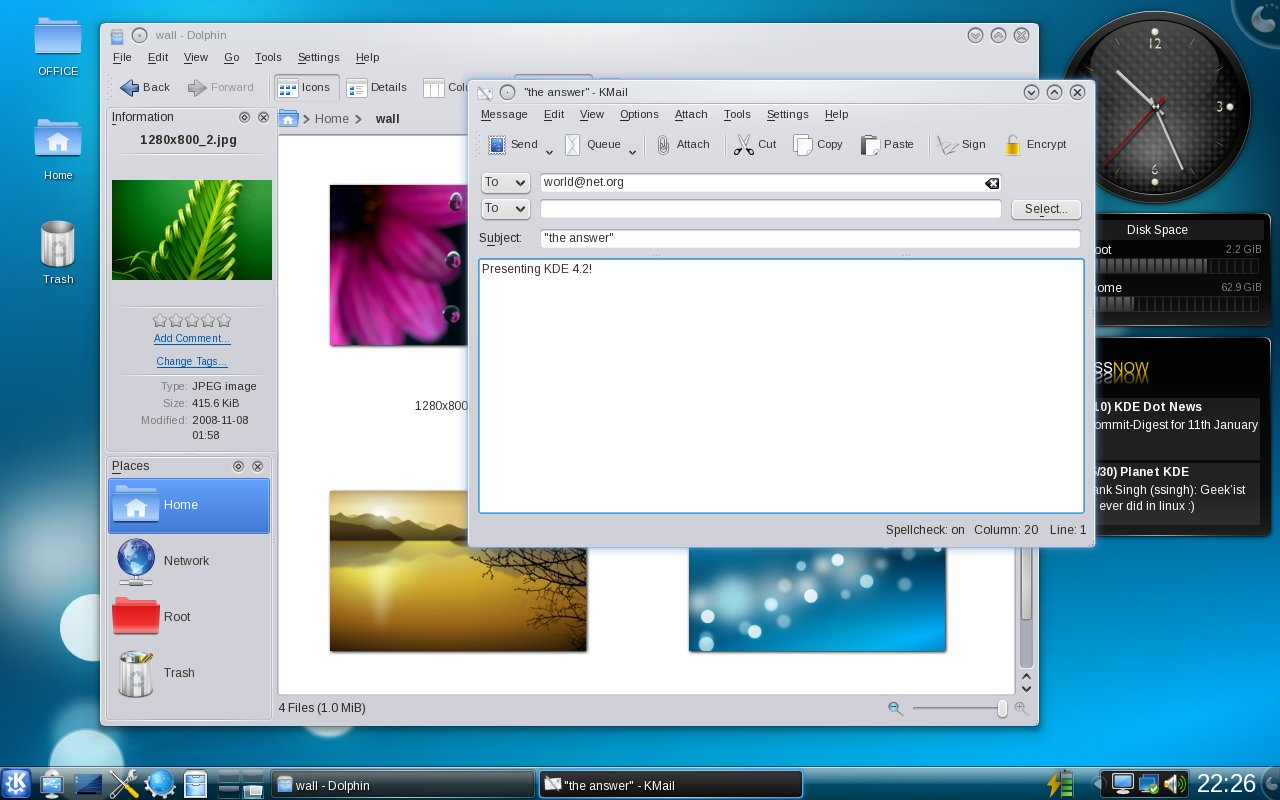
\includegraphics[width=\linewidth]{images/kde4.jpeg}
	\caption{KDE Version 4.2 \cite{geschichtekde}}
	\label{fig:kdeversion4}
\end{figure}

Zusammen mit KDE 4 begann die Community mit einem zeit-basierten Release-Plan. Feature-Releases wurden demnach jedes halbe Jahr und Bugfix-Releases jeden Monat veröffentlicht. Die halbjährlich veröffentlichten Softwarekomponenten waren fortan unter dem Namen \textit{KDE Software Compilation (KDE SC)} bekannt. \cite{geschichtekde}

\subsubsection{KDE Plasma 5}
KDE Plasma ist die 5. Generation der KDE Arbeitsumgebung und stellt heute das Hauptprodukt der Community dar. Sie wurde am 15. Juli 2014 veröffentlicht. Durch den Wesel auf Qt 5 wurde die Grafikausgabe auf Open GL umgestellt und bot viele neue visuelle Features. \cite{kdeplasma5} Weitere Informationen zu KDE Plasma 5 werden in Abschnitt \ref{plasma5} beschrieben. Abbildung \ref{fig:kdeversion5} zeigt ein Bild der Arbeitsumgebung.

\begin{figure}[h]
	\centering
	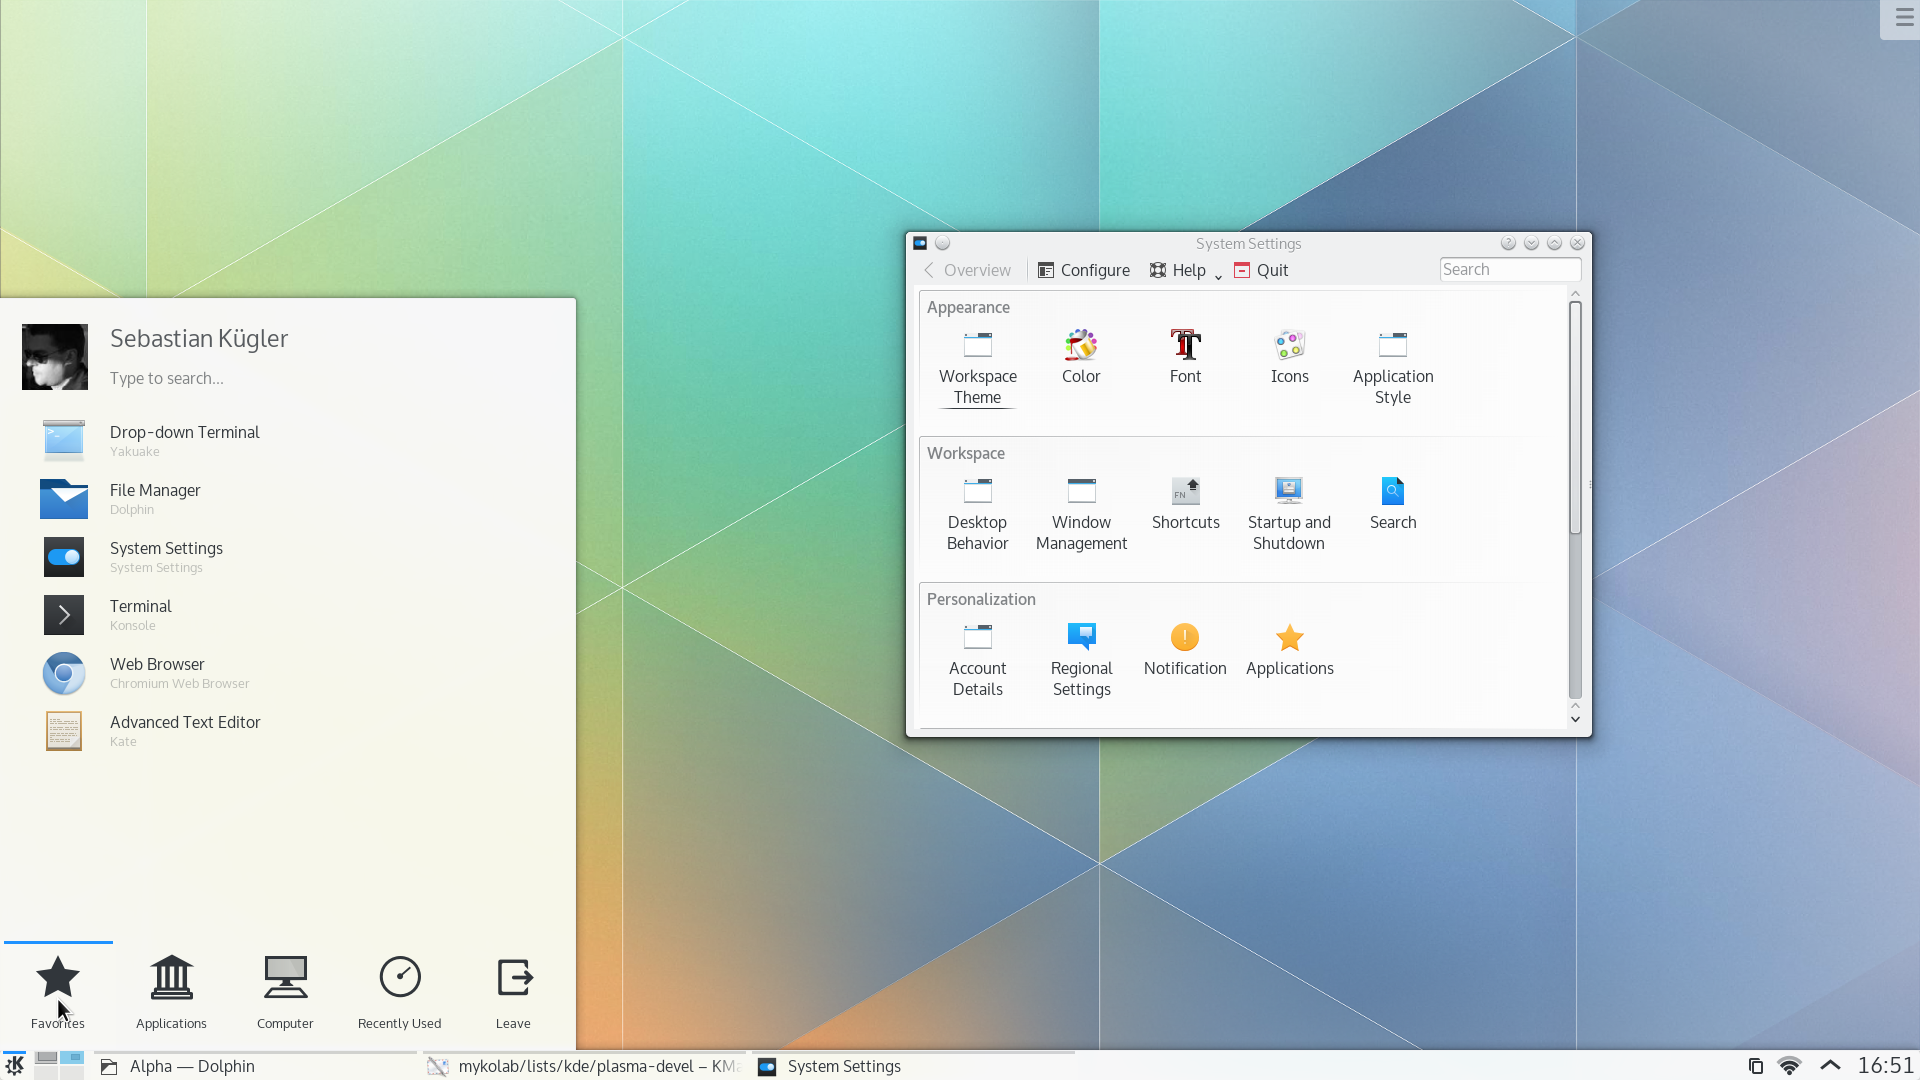
\includegraphics[width=\linewidth]{images/kde5.png}
	\caption{KDE Version 5.0 \cite{kdeplasma5}}
	\label{fig:kdeversion5}
\end{figure}
